\chapter{Experimento $\nu$-Angra}\label{cap:experimento}
\vspace{-2cm}

O experimento $\nu$-Angra tem como objetivo a criação de um detector de superfície capaz de detectar antineutrinos advindos da queima de combustível nuclear através da relação entre potência térmica dissipada e a taxa de eventos de antineutrinos registrados pelo detector.

O detector utiliza da radiação de Cherenkov (apêndice \ref{apdx:cherenkov}) na água para fazer a contagem de eventos. Afim de coletar os fótons gerados são utilizados 40 PMTs, do modelo Hamamatsu R5912.

Como o detector é de superfície, para melhorar a relação sinal ruído ele é posicionado a poucos metros do reator nuclear da usina Angra 2 em um contêiner-laboratório, como pode ser visto na Figura \ref{fig:angra}.

\begin{figure}[H]
	\centering
	\includegraphics[width=10cm]{textuais/experimento/figuras/angra.png}
	\caption{Detector posicionado ao lado do reator nuclear da usina Angra 2}
	\label{fig:angra}
\end{figure}

\section{Reator nuclear da usina Angra 2}

O reator nuclear da usina Angra 2 é do tipo \ac{PWR}, no qual o sistema de refrigeração é baseado em água bombeada em alta pressão no núcleo do reator, onde é aquecida pela fissão nuclear, que passa por um gerador de se vapor e move turbinas, transformando energia térmica em energia elétrica. Alguns sub-processos da geração térmica nuclídeos gerados pela fissão nuclear, que através do decaimento beta, formam antineutrinos, que são espalhados em todas as direções.

\section{O detector $\nu$-Angra}

O detector utilizado dispõe de três sistemas principais que podem ser vistos na Figura \ref{fig:detector} e serão discutidos em suas sub-sessões, possui volume aproximado de $13$ m$^3$, sendo apenas $\dfrac{1}{10}$ do volume para o detector alvo e o resto dividido em \emph{shielding} e o sistema de veto, ambos para proteger o detector de ruído de fundo como raios cósmicos ou nêutrons.

\begin{figure}[H]
    \centering
    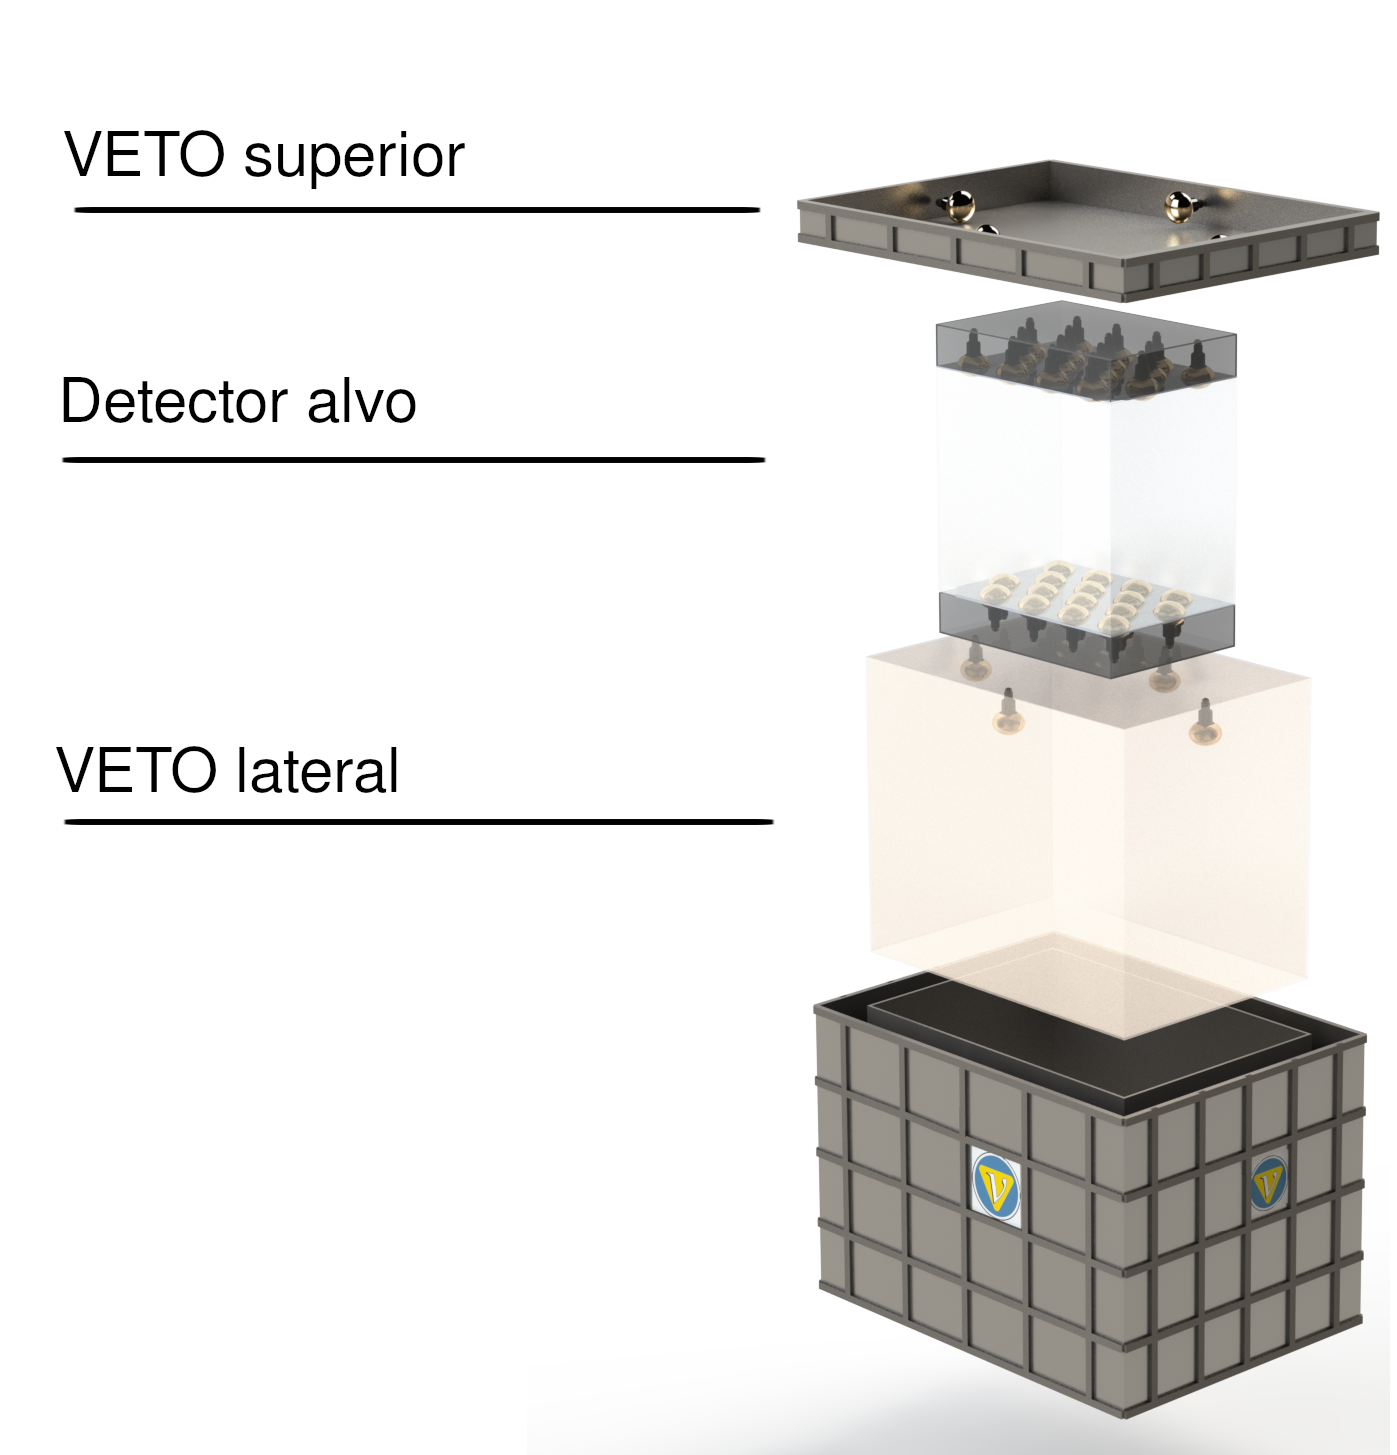
\includegraphics[width=11cm]{textuais/experimento/figuras/detector.png}
    \caption{Vista explodida do detector}
    \label{fig:detector}
\end{figure}

\subsection{Sistemas de \emph{VETO}}

Como o detector $\nu$-Angra é um detector de superfície ele não está imune à radiação advinda do cosmos, se fazendo necessário uma camada de veto para detecção de ruídos de fundo afim de selecionar apenas os eventos de antineutrinos. Cada camada de \emph{VETO} têm 4 PMTs, sendo as do \emph{VETO} superior sendo posicionadas no ponto central de cada aresta, enquanto as do \emph{VETO} lateral ficam na parte superior das faces laterais do detector, somando-se 8 PMTs. O veto lateral é revestido com uma fina camada de aço para bloquear principalmente nêutrons. \url{http://lsd.cbpf.br/doc/dissertacoes/TeseDoutorado_DionRibeiro.2019_05_07.pdf}

\subsection{Detector alvo}

Como eventos de antineutrinos são de baixa energia, para melhor leitura dos eventos, o alvo apresenta 16 PMTs na sua parte inferior e 16 na parte superior, ele é preenchido com um cintilador dopado com gadolínio afim de aumentar o número de partículas livres que interagem com antineutrinos através do processo de decaimento beta-inverso. O detector alvo têm volume aproximado de $1$  m$^3$, e tem a carcaça feita de polipropileno.



\begin{equation}
n \rightarrow p + e^- + \bar{\nu}_e 
\end{equation}

\section{Eletrônicas de \emph{front-end} e aquisição}

Para fazer a aquisição dos sinais das PMTs, o detector dispõe de circuitos eletrônicos para condicionamento dos sinais, chamado de \emph{front-end}, e um sistema de aquisição dos dados, chamado de \ac{NDAQ}. Cada PMT tem uma \emph{front-end} conectada à saída de sinal que então estão ligadas em cada um dos oito canais de cada NDAQ, fazendo-se assim $40$ placas de \emph{front-end} e $5$ NDAQs para a aquisição de todas as PMTs do detector.

Durante todo o tempo os sinais das PMTs são salvos em uma fila do tipo FIFO (do inglês \emph{first in first out}) nas NDAQs, quando um sinal é detectado o conteúdo das \emph{fifos} é esvaziado, digitalizado pelas NDAQs e salvo em um arquivo para análise prévia.

